% !TEX TS-program = pdflatex
% !TEX encoding = UTF-8 Unicode

% This is a simple template for a LaTeX document using the "article" class.
% See "book", "report", "letter" for other types of document.

\documentclass[11pt]{article} % use larger type; default would be 10pt

\usepackage[utf8]{inputenc} % set input encoding (not needed with XeLaTeX)

%%% Examples of Article customizations
% These packages are optional, depending whether you want the features they provide.
% See the LaTeX Companion or other references for full information.

%%% PAGE DIMENSIONS
\usepackage{geometry} % to change the page dimensions
\geometry{a4paper} % or letterpaper (US) or a5paper or....
% \geometry{margin=2in} % for example, change the margins to 2 inches all round
% \geometry{landscape} % set up the page for landscape
%   read geometry.pdf for detailed page layout information

\usepackage{graphicx} % support the \includegraphics command and options
\usepackage{float}

% \usepackage[parfill]{parskip} % Activate to begin paragraphs with an empty line rather than an indent

%%% PACKAGES
\usepackage{booktabs} % for much better looking tables
\usepackage{array} % for better arrays (eg matrices) in maths
\usepackage{paralist} % very flexible & customisable lists (eg. enumerate/itemize, etc.)
\usepackage{verbatim} % adds environment for commenting out blocks of text & for better verbatim
\usepackage{subfig} % make it possible to include more than one captioned figure/table in a single float
% These packages are all incorporated in the memoir class to one degree or another...

%%% HEADERS & FOOTERS
\usepackage{fancyhdr} % This should be set AFTER setting up the page geometry
\pagestyle{fancy} % options: empty , plain , fancy
\renewcommand{\headrulewidth}{0pt} % customise the layout...
\lhead{}\chead{}\rhead{}
\lfoot{}\cfoot{\thepage}\rfoot{}

%%% SECTION TITLE APPEARANCE
\usepackage{sectsty}
\allsectionsfont{\sffamily\mdseries\upshape} % (See the fntguide.pdf for font help)
% (This matches ConTeXt defaults)

%%% ToC (table of contents) APPEARANCE
\usepackage[nottoc,notlof,notlot]{tocbibind} % Put the bibliography in the ToC
\usepackage[titles,subfigure]{tocloft} % Alter the style of the Table of Contents
\renewcommand{\cftsecfont}{\rmfamily\mdseries\upshape}
\renewcommand{\cftsecpagefont}{\rmfamily\mdseries\upshape} % No bold!

%% Automata
\usepackage{pgf}
\usepackage{tikz}
\usetikzlibrary{arrows,automata,positioning}
\usepackage{tikz-qtree}

%% Rotate text in tables etc.
\def\rot{\rotatebox}

%%% END Article customizations


%%% The "real" document content comes below...

\title{Exercises Compiler Construction}
\author{Martijn Verkleij (s1466895) \& Wouter Bos (s1606824)}
%\date{} % Activate to display a given date or no date (if empty),
         % otherwise the current date is printed 

\begin{document}
\maketitle

\section*{Exercise 1}

\bgroup
\def\arraystretch{1.5}
\begin{tabular}{lp{10cm}}
\textbf{Term} & \textbf{Meaning} \\
\hline
AST
& Abstract Syntax Tree. It only shows the abstract syntactic structure of the source code. A parse tree retains all information of the source code, while an AST only shows the information related to the syntactic structure. \\

DAG
& Directed Acyclic Graph. It is a directed graph with no directed cycles. There is no way to start at a node n and follow a sequence of edges that eventually loops back to n again. \\

Basic Block
& A maximal length sequence of straightline, or branch-free, code. A basic block is a sequence of operations that always execute together, unless an operation raises an exception. Control always enters a basic block at its first operation and exits at its last operation. \\

CFG
& Context-free Grammar. A formal grammar in which every production rule is of the form V $\rightarrow$ w, where V is a single nonterminal and w is a string of terminals and nonterminals or empty. \\

& Control Flow Graph. A representation of all paths that might be transversed during the execution of a program. \\

Dependence Graph
& A directed graph representing the dependencies of objects towards each other. \\

Call Graph
& A flow graph that represents calling relationships between subroutines in a program. \\

SSA
& Static Single Assignment. Each variable is assigned exactly once, and each variable is defined before it is used. \\

Symbol Table
& A data structure where each identifier is associated with information relating to its declaration or appearance in the program. \\

\hline
\end{tabular}
\egroup

\section*{Exercise 2.1}
\begin{tikzpicture}
\node (A) {1};
\node (B) [below of = A]{2};
\node (C) [below of = B]{3};
\node (D) [below of = C]{4};
\node (E) [below of = D]{5};
\node (F) [below of = E]{6};
\node (G) [below of = F]{7};
\node (J) [left of = E]{10};

\draw[->] (A) -- (B);
\draw[->] (B) -- (C);
\draw[->] (C) -- (D);
\draw[->] (D) -- (E);
\draw[->] (E) -- (F);
\draw[->] (F) -- (G);
\draw[->] (F) .. controls +(right:25pt) and +(right:25pt) .. (D);
\draw[->] (G) .. controls +(right:55pt) and +(right:55pt) .. (D);
\draw[->] (D.west) .. controls +(left:15pt) and +(up:15pt) .. (J.north);

\end{tikzpicture}

\section*{Exercise 2.2}
(1, 2, 3), (5, 6)

\section*{Exercise 2.3}
1, 2, 3

\section*{Exercise 3.1}
\begin{tikzpicture}
\node (A) {1};
\node (B) [below of = A]{2};
\node (C) [below of = B]{3};
\node (D) [below of = C]{4};
\node (E) [below of = D]{5};
\node (F) [below of = E]{6};
\node (G) [below right of = F]{7};
\node (I) [below left of = G]{9};
\node (K) [left of = E]{11};

\draw[->] (A) -- (B);
\draw[->] (B) -- (C);
\draw[->] (C) -- (D);
\draw[->] (E) -- (D);
\draw[->] (E) -- (F);
\draw[->] (F) -- (G);
\draw[->] (F) -- (I);
\draw[->] (G) .. controls +(right:25pt) and +(right:25pt) .. (E);
\draw[->] (I) .. controls +(right:55pt) and +(right:55pt) .. (E);
\draw[->] (D.west) .. controls +(left:15pt) and +(up:15pt) .. (K.north);

\end{tikzpicture}

\section*{Exercise 3.2}
(1, 2, 3)

\section*{Exercise 3.3}
1, 2, 3

\section*{Exercise 4}
The difference between the computed and reasoned about solution is the inclusion of exit nodes on decision nodes like while loops. These are used to be able to differentiate between the desired bahaviors, and they provide a placeholder for the next statement that is not yet parsed at that time.


\section*{Exercise 7}
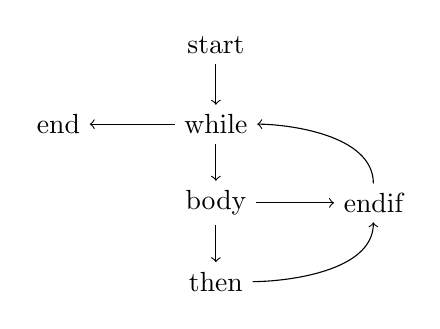
\begin{tikzpicture}
\node (A) {start};
\node (B) [below of = A]               {while};
\node (C) [below of = B]               {body};
\node (D) [below of = C]               {then};
\node (E) [right of = C, xshift = 1cm] {endif};
\node (F) [left of  = B, xshift = -1cm]{end};

\draw[->] (A) -- (B);
\draw[->] (B) -- (C);
\draw[->] (C) -- (D);
\draw[->] (B) -- (F);
\draw[->] (C) -- (E);
\draw[->] (D) .. controls +(right:25pt) and +(down:25pt) .. (E);
\draw[->] (E) .. controls +(up:25pt) and +(right:25pt) .. (B);
\end{tikzpicture}

\end{document}
